\section{Experiments}
\label{sec:experiments}

\subsection{Experimental Setup}
The experiments use the current MATLAB implementation of the RCH-MT-MMP pipeline.
 The main benchmark is a \(10\,\mathrm{m}\times 10\,\mathrm{m}\) indoor 
 tabletop-service scene with 16 rectangular tables arranged in four rows and 36 tabletop task points distributed 
 over the table surfaces. This setting tests the decision layer that precedes arm execution: 
 the robot must determine which collision-free docking poses make the tabletop tasks reachable, 
 select enough poses to cover all tasks, and connect the selected poses with a global route.

Figure~\ref{fig:main_scenario_scene} shows the main scene and the resulting plan.
 Gray rectangles denote tables, green circles denote tabletop task points, 
 orange triangles denote selected docking poses, the blue polyline denotes the global navigation path, 
 and the red star denotes the start state. Several tables require more than one docking pose because task points on different sides
  cannot all be reached from a single base placement under the dual-arm reachability and clearance constraints. 
  The default global planner is A*, and all reported submission-level data are generated from the `submission' experiment mode.

\begin{figure}[!t]
    \centering
    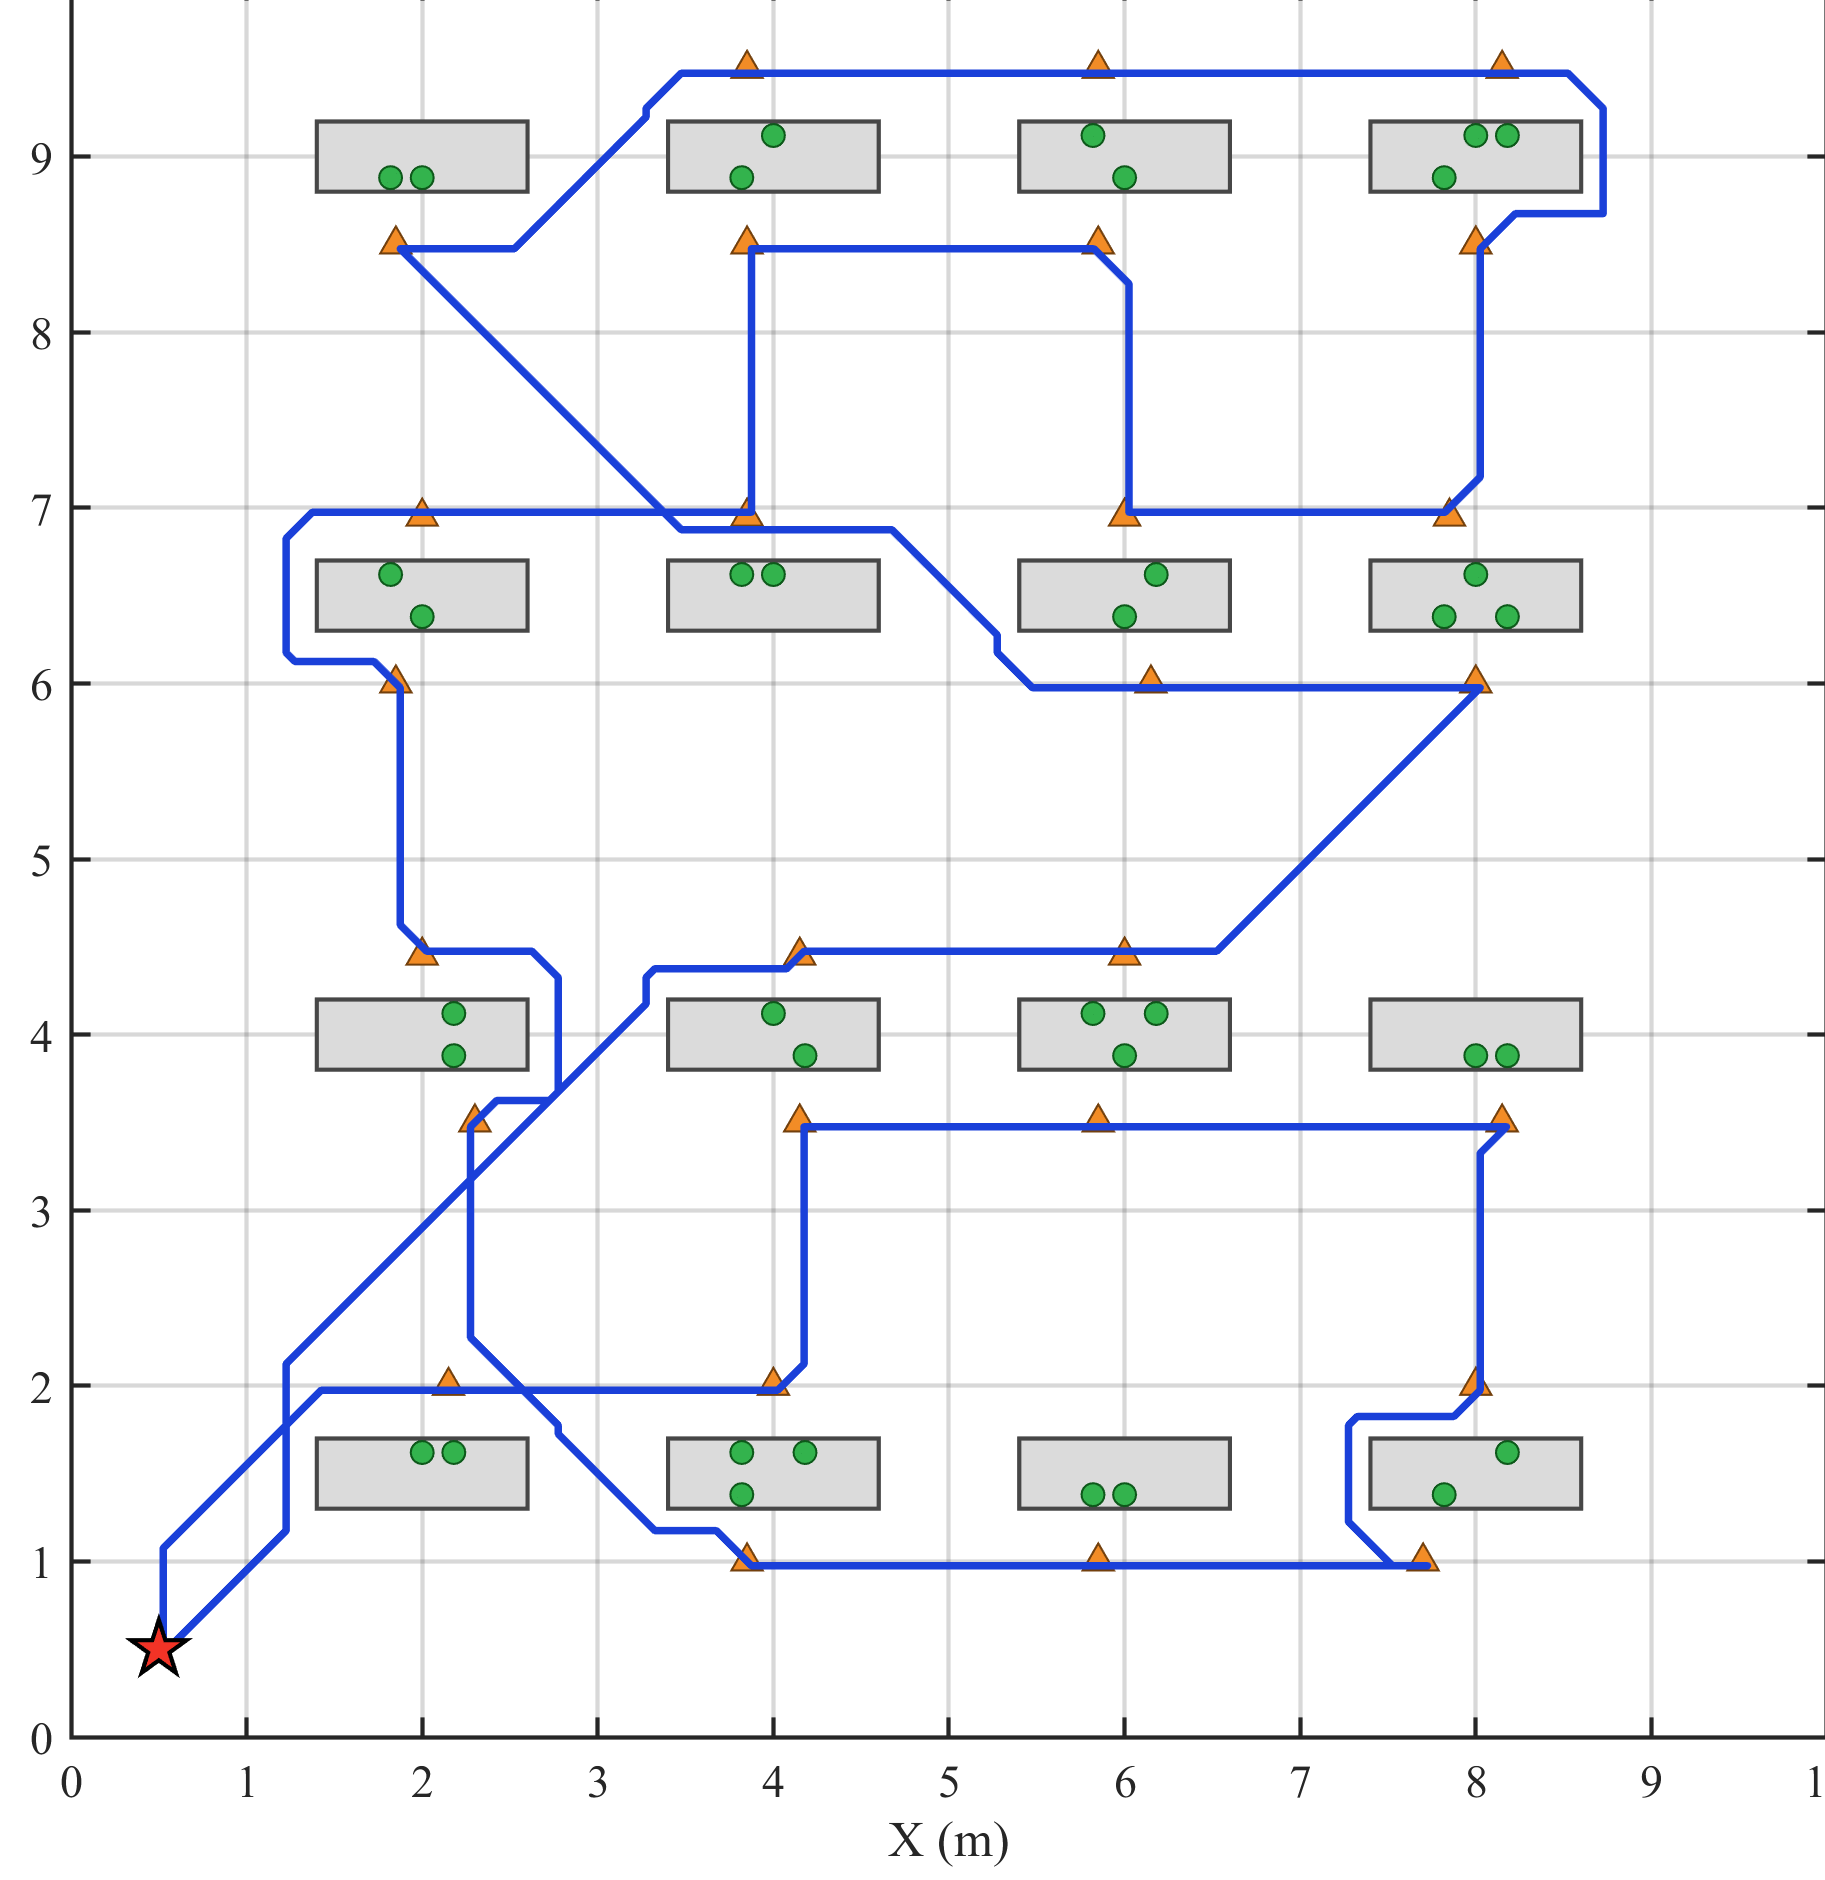
\includegraphics[width=0.88\columnwidth]{results/figures/tac_submission/png/fig_main_scenario_scene.png}
    \caption{Experimental configuration of the main tabletop-service scene. The \(10\,\mathrm{m}\times10\,\mathrm{m}\) 
    map contains 16 rectangular tables and 36 tabletop task points. Green circles mark tasks, 
    orange triangles mark selected collision-free docking poses, the red star marks the start state,
     and the blue polyline is the A*-planned route.}
    \label{fig:main_scenario_scene}
\end{figure}

\begin{figure*}[!t]
    \centering
    \begin{minipage}[t]{0.49\textwidth}
        \centering
        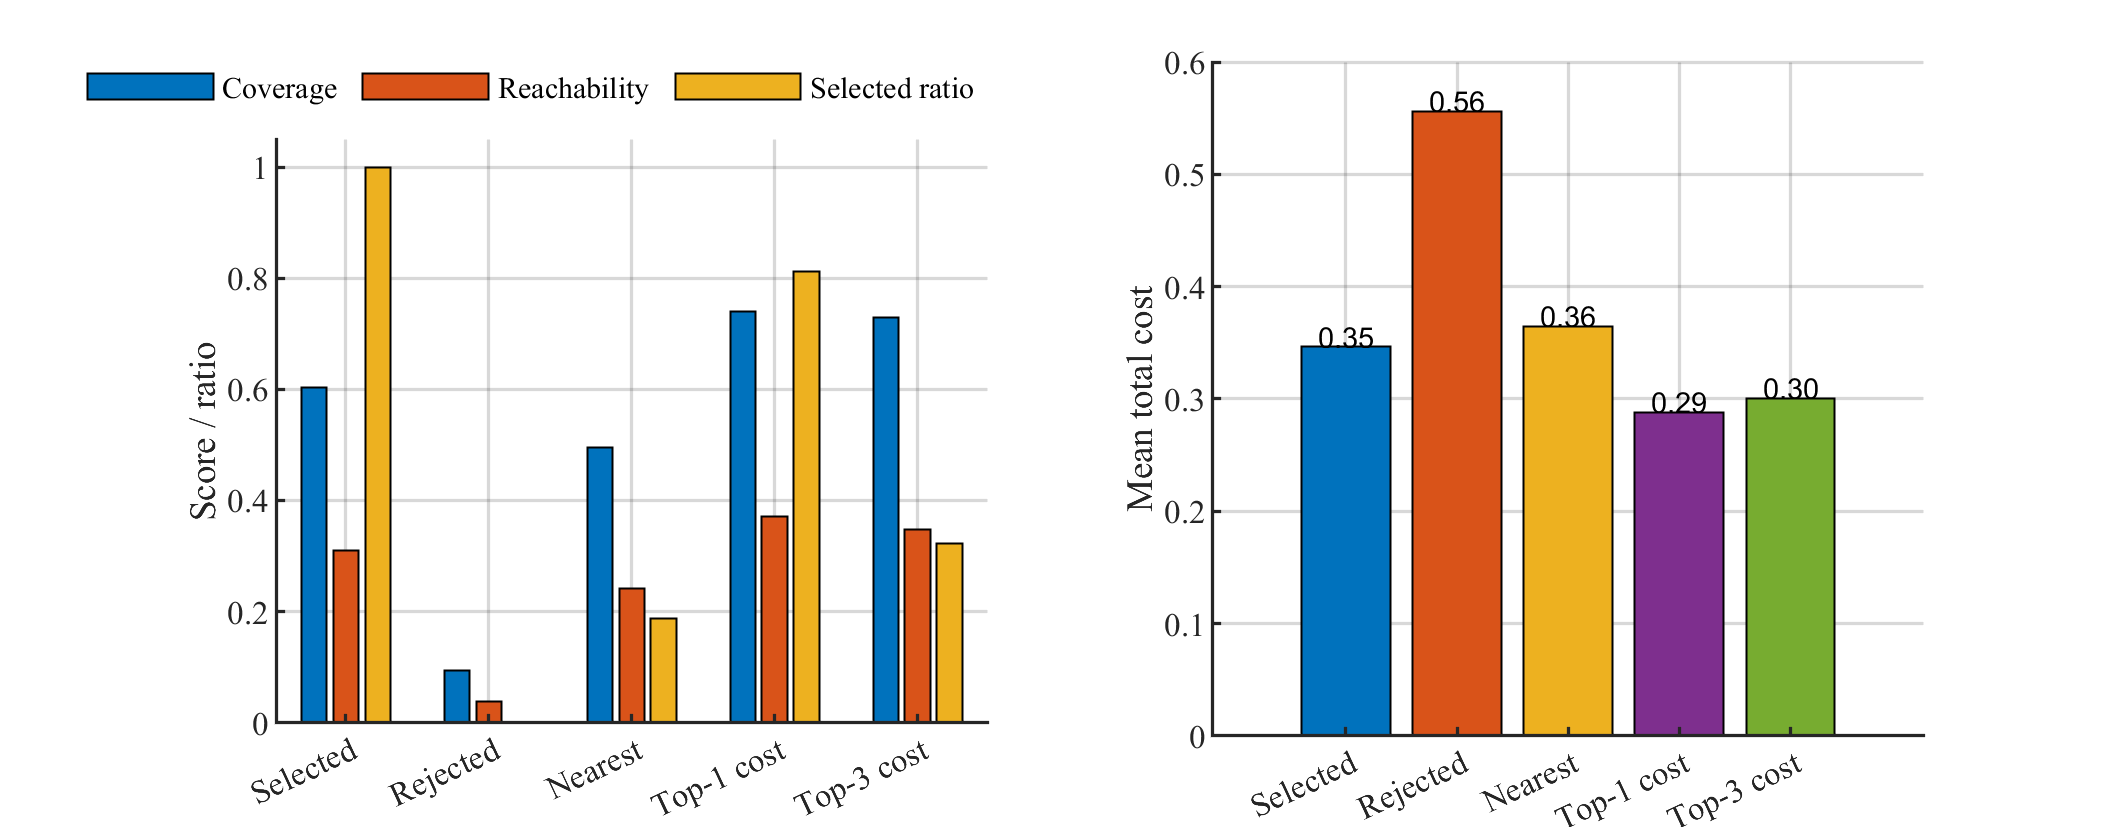
\includegraphics[width=\linewidth]{results/figures/tac_submission/png/fig_candidate_quality.png}
        \vspace{0.1em}
        \small (a) Candidate docking-pose quality.
    \end{minipage}\hfill
    \begin{minipage}[t]{0.49\textwidth}
        \centering
        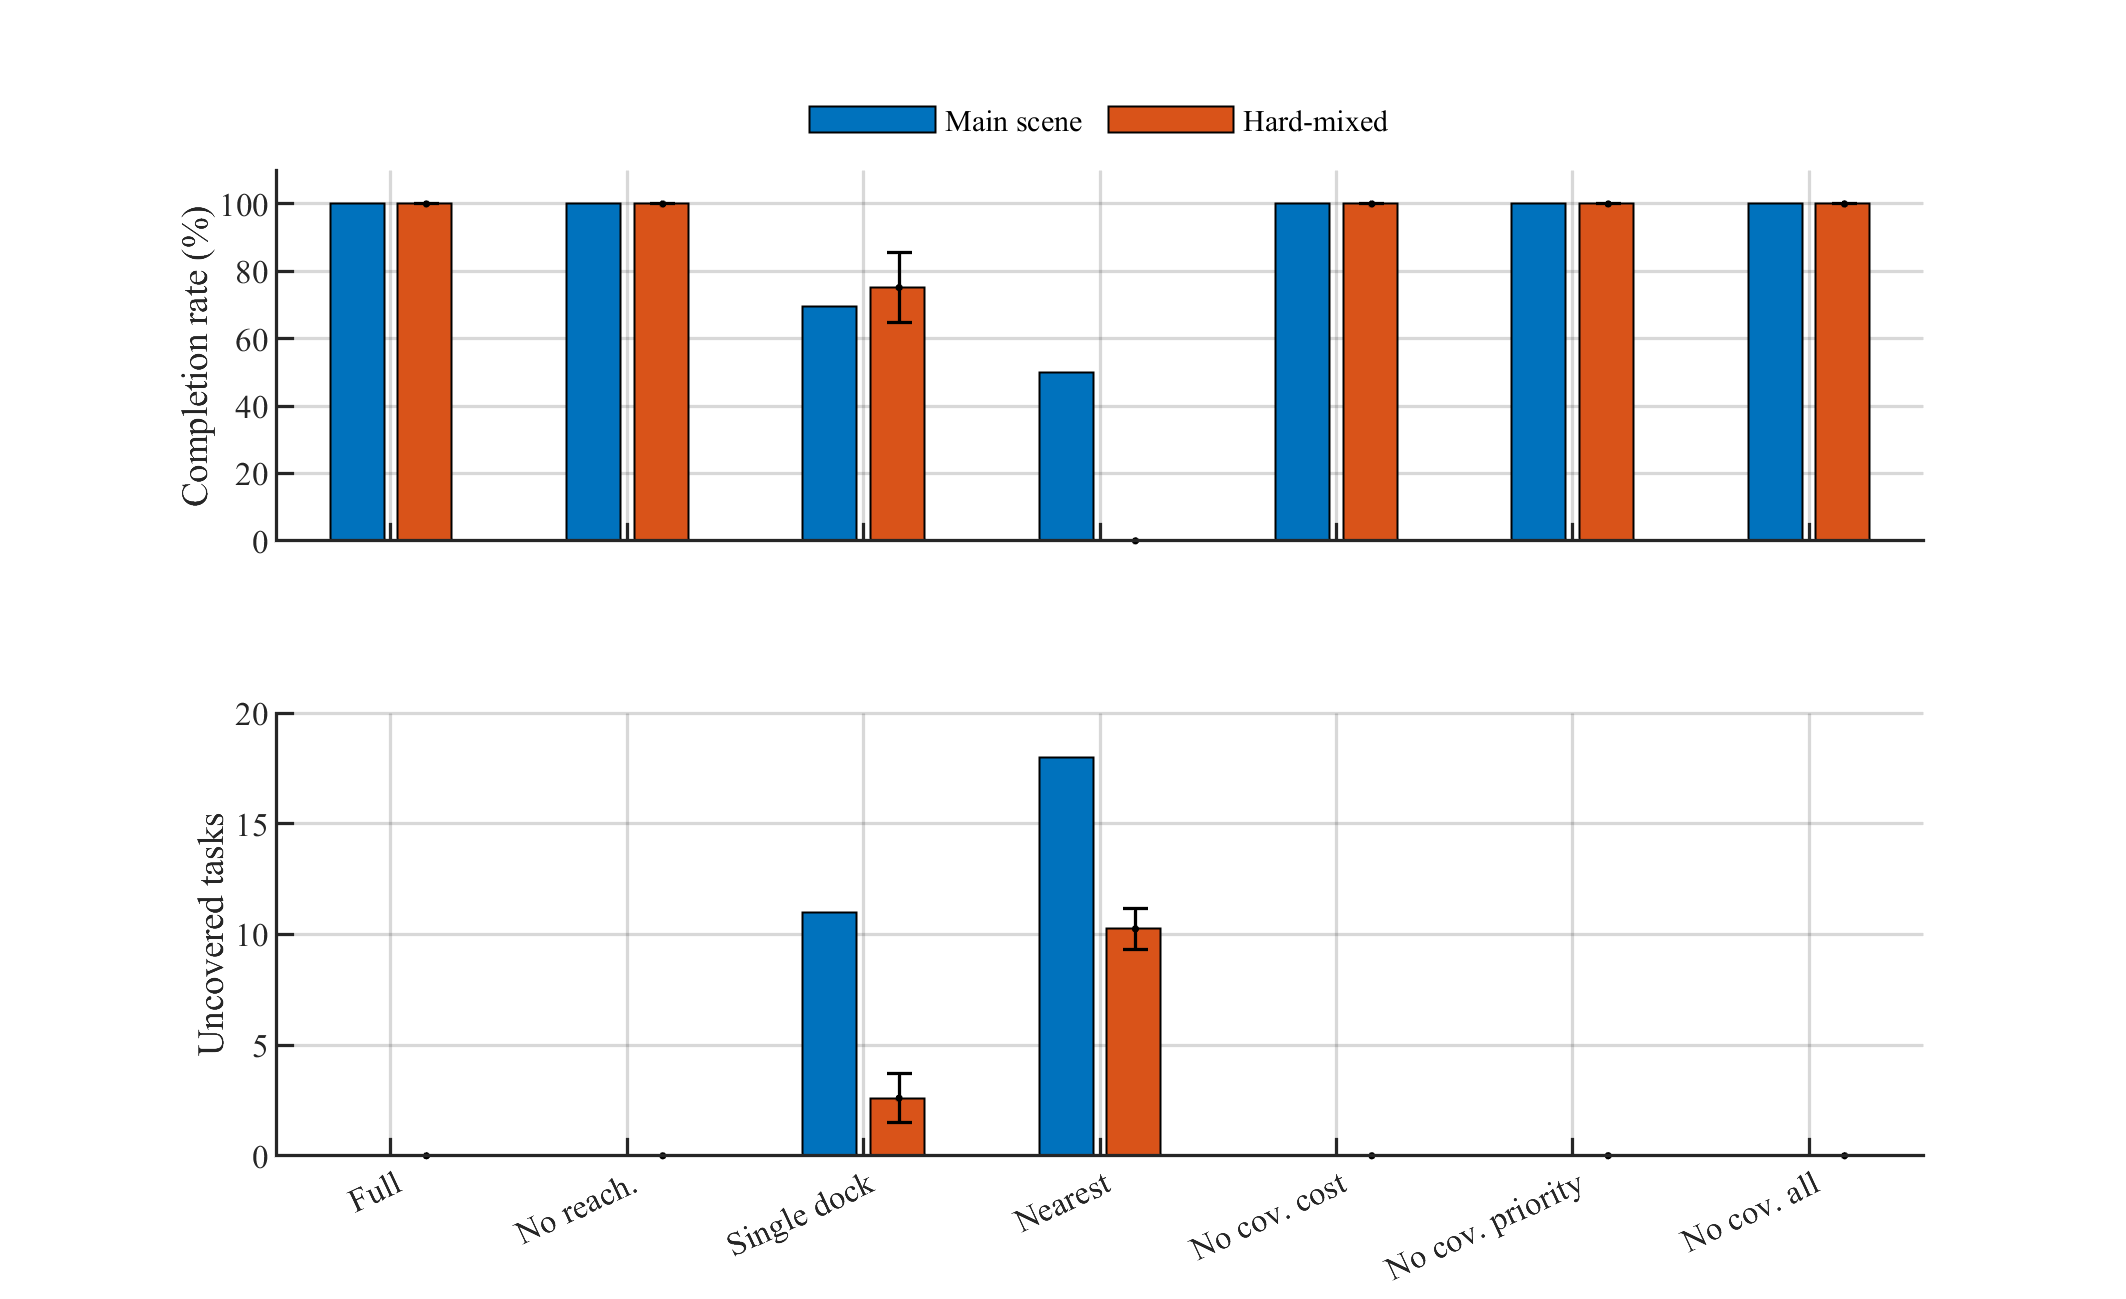
\includegraphics[width=\linewidth]{results/figures/tac_submission/png/fig_ablation_completion.png}
        \vspace{0.1em}
        \small (b) Main and hard-mixed ablations.
    \end{minipage}
    \caption{Candidate quality and ablation evidence. 
    (a) Selected poses provide stronger coverage and reachability than rejected candidates.
     (b) Single-docking and nearest-docking variants leave uncovered tasks 
     because they ignore either multi-side coverage or reachability-aware docking quality.}
    \label{fig:quality_ablation}
\end{figure*}

\begin{table}[!t]
\centering
\caption{Main scenario result.}
\label{tab:main}
\begin{tabular}{lr}
\toprule
Metric & Value \\
\midrule
Tasks & 36 \\
Completed tasks & 36 \\
Completion rate & 100.00\% \\
Selected docking poses & 27 \\
Task path length & 57.34 m \\
Return path length & 5.95 m \\
Total path length & 63.29 m \\
Planning time & 28.85 s \\
Estimated execution time & 789.79 s \\
\bottomrule
\end{tabular}
\end{table}

\subsection{Main Scenario and Candidate Quality}
    Table~\ref{tab:main} reports the numerical result for the scene in Figure~\ref{fig:main_scenario_scene}. 
    The full method completes all 36 tasks with 27 selected docking poses and a total route length of 63.29 m. 
    This result supports the central claim that tabletop service requirements can first be converted into 
    reachability-aware docking decisions and then connected by a replaceable global path planner. 
    The relatively large number of selected poses is not a failure of path shortening; it reflects 
    the manipulation constraint that some tables require service from multiple sides to cover all task points.

    Figure~\ref{fig:quality_ablation}(a) compares selected and rejected candidate docking poses. 
    Selected candidates have mean coverage ratio 0.604 and mean reachability score 0.310,
    while rejected candidates have mean coverage ratio 0.094 and mean reachability score 0.038. 
    This gap indicates that the scoring function selects poses that are meaningfully better for 
    manipulation coverage rather than merely close in navigation space.

\subsection{Ablation Studies}
Figure~\ref{fig:quality_ablation}(b) and Table~\ref{tab:baseline_submission} evaluate the necessity of reachability-aware multi-docking. 
In the main scenario, the full method reaches 100.00\% completion, while single docking per table reaches 69.44\% and nearest docking reaches 50.00\%. 
In the submission-level baseline comparison over 1120 records, the full method keeps 100.00\% mean completion, single docking reaches 73.73\%, 
and nearest docking reaches 25.59\%. 
These failures show that shorter or simpler docking choices are not sufficient when task coverage is constrained by dual-arm reachability.

\begin{table}[!t]
\centering
\caption{Submission-level baseline comparison.}
\label{tab:baseline_submission}
\footnotesize
\setlength{\tabcolsep}{3.2pt}
\begin{tabular}{@{}lrrrrr@{}}
\toprule
Method & Trials & Completion & Uncovered & Docks & Time \\
 & & (\%) & & & (s) \\
\midrule
Full & 140 & 100.00 & 0.00 & 10.99 & 12.28 \\
Single dock & 140 & 73.73 & 4.49 & 6.43 & 11.10 \\
Nearest & 120 & 25.59 & 10.99 & 6.83 & 11.17 \\
Set-cover greedy & 140 & 100.00 & 0.00 & 11.11 & 10.62 \\
Random feasible & 140 & 100.00 & 0.00 & 15.02 & 13.05 \\
\bottomrule
\end{tabular}
\end{table}

\subsection{Hard Scenarios and Stress Boundaries}
 The hard-scenario suite includes normal, hard-corner, hard-two-side, hard-reach-boundary, 
 and hard-mixed task distributions. The full method maintains complete coverage in all five distributions in the generated summary data. 
 Figure~\ref{fig:hard_stress}(a) shows that nearest and single-docking baselines degrade sharply under hard distributions, 
 which supports the need for multi-docking coverage.
 Figure~\ref{fig:hard_stress}(b) reports sensitivity to table spacing, reachability threshold, task density, and candidate density. 
 The lowest mean completion in the stress summary is 96.92\% at reachability threshold 0.5,
  while most settings remain at full completion.

\begin{figure*}[!t]
    \centering
    \begin{minipage}[t]{0.49\textwidth}
        \centering
        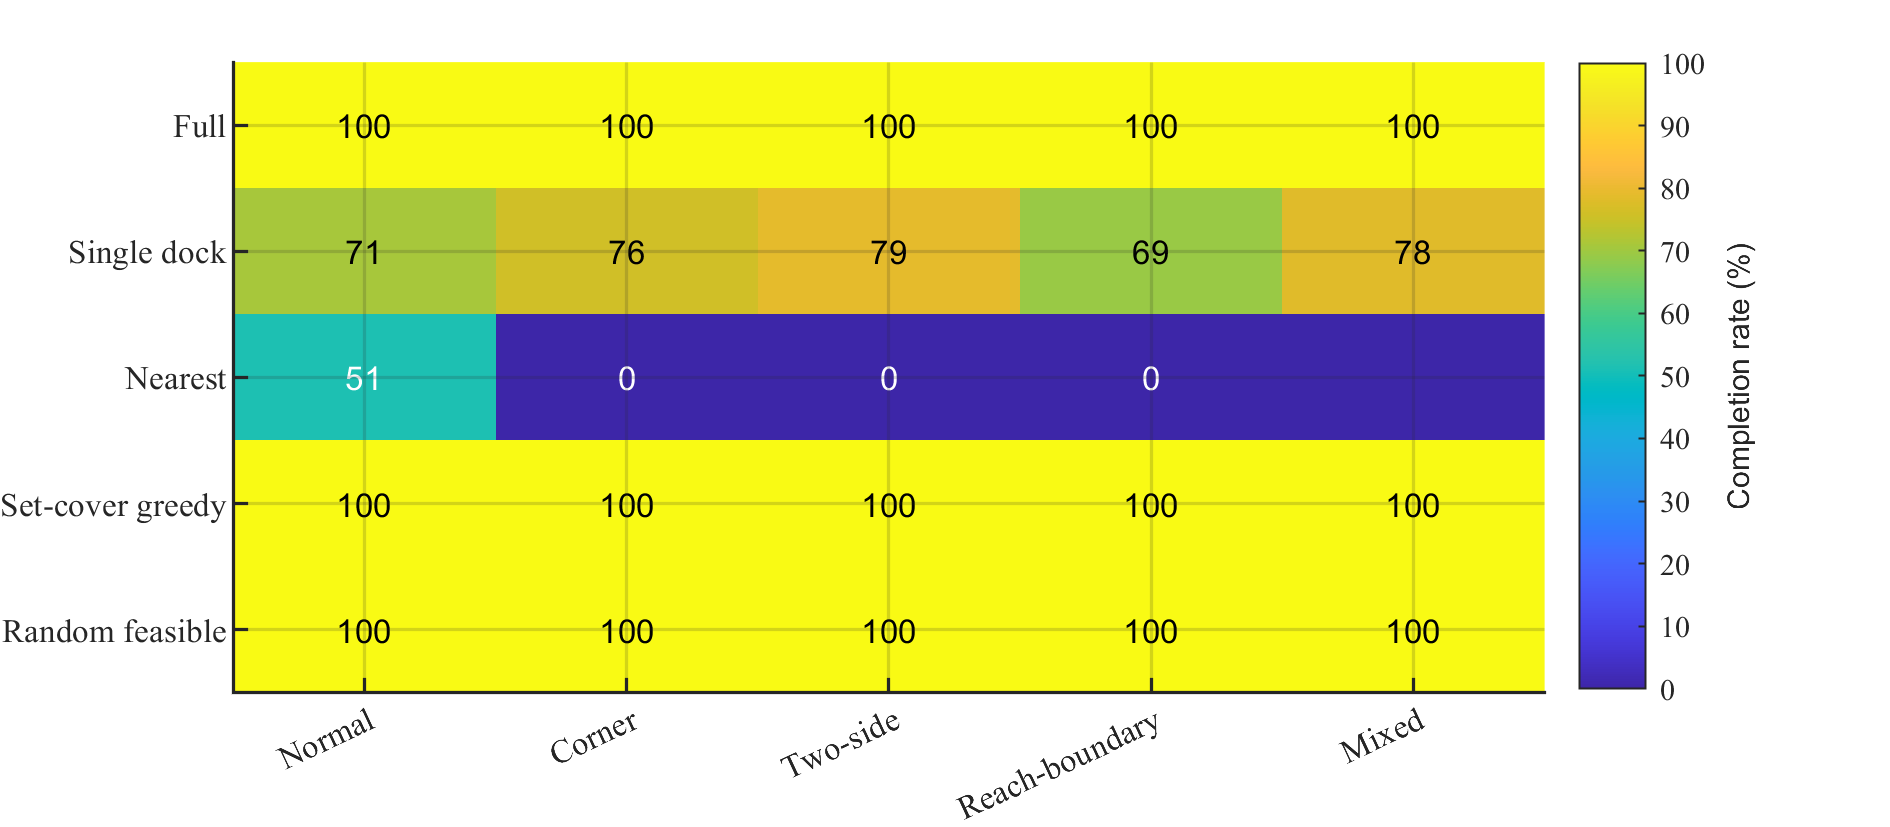
\includegraphics[width=\linewidth]{results/figures/tac_submission/png/fig_hard_scenario_heatmap.png}
        \vspace{0.2em}
        \small (a) Completion across hard distributions.
    \end{minipage}\hfill
    \begin{minipage}[t]{0.49\textwidth}
        \centering
        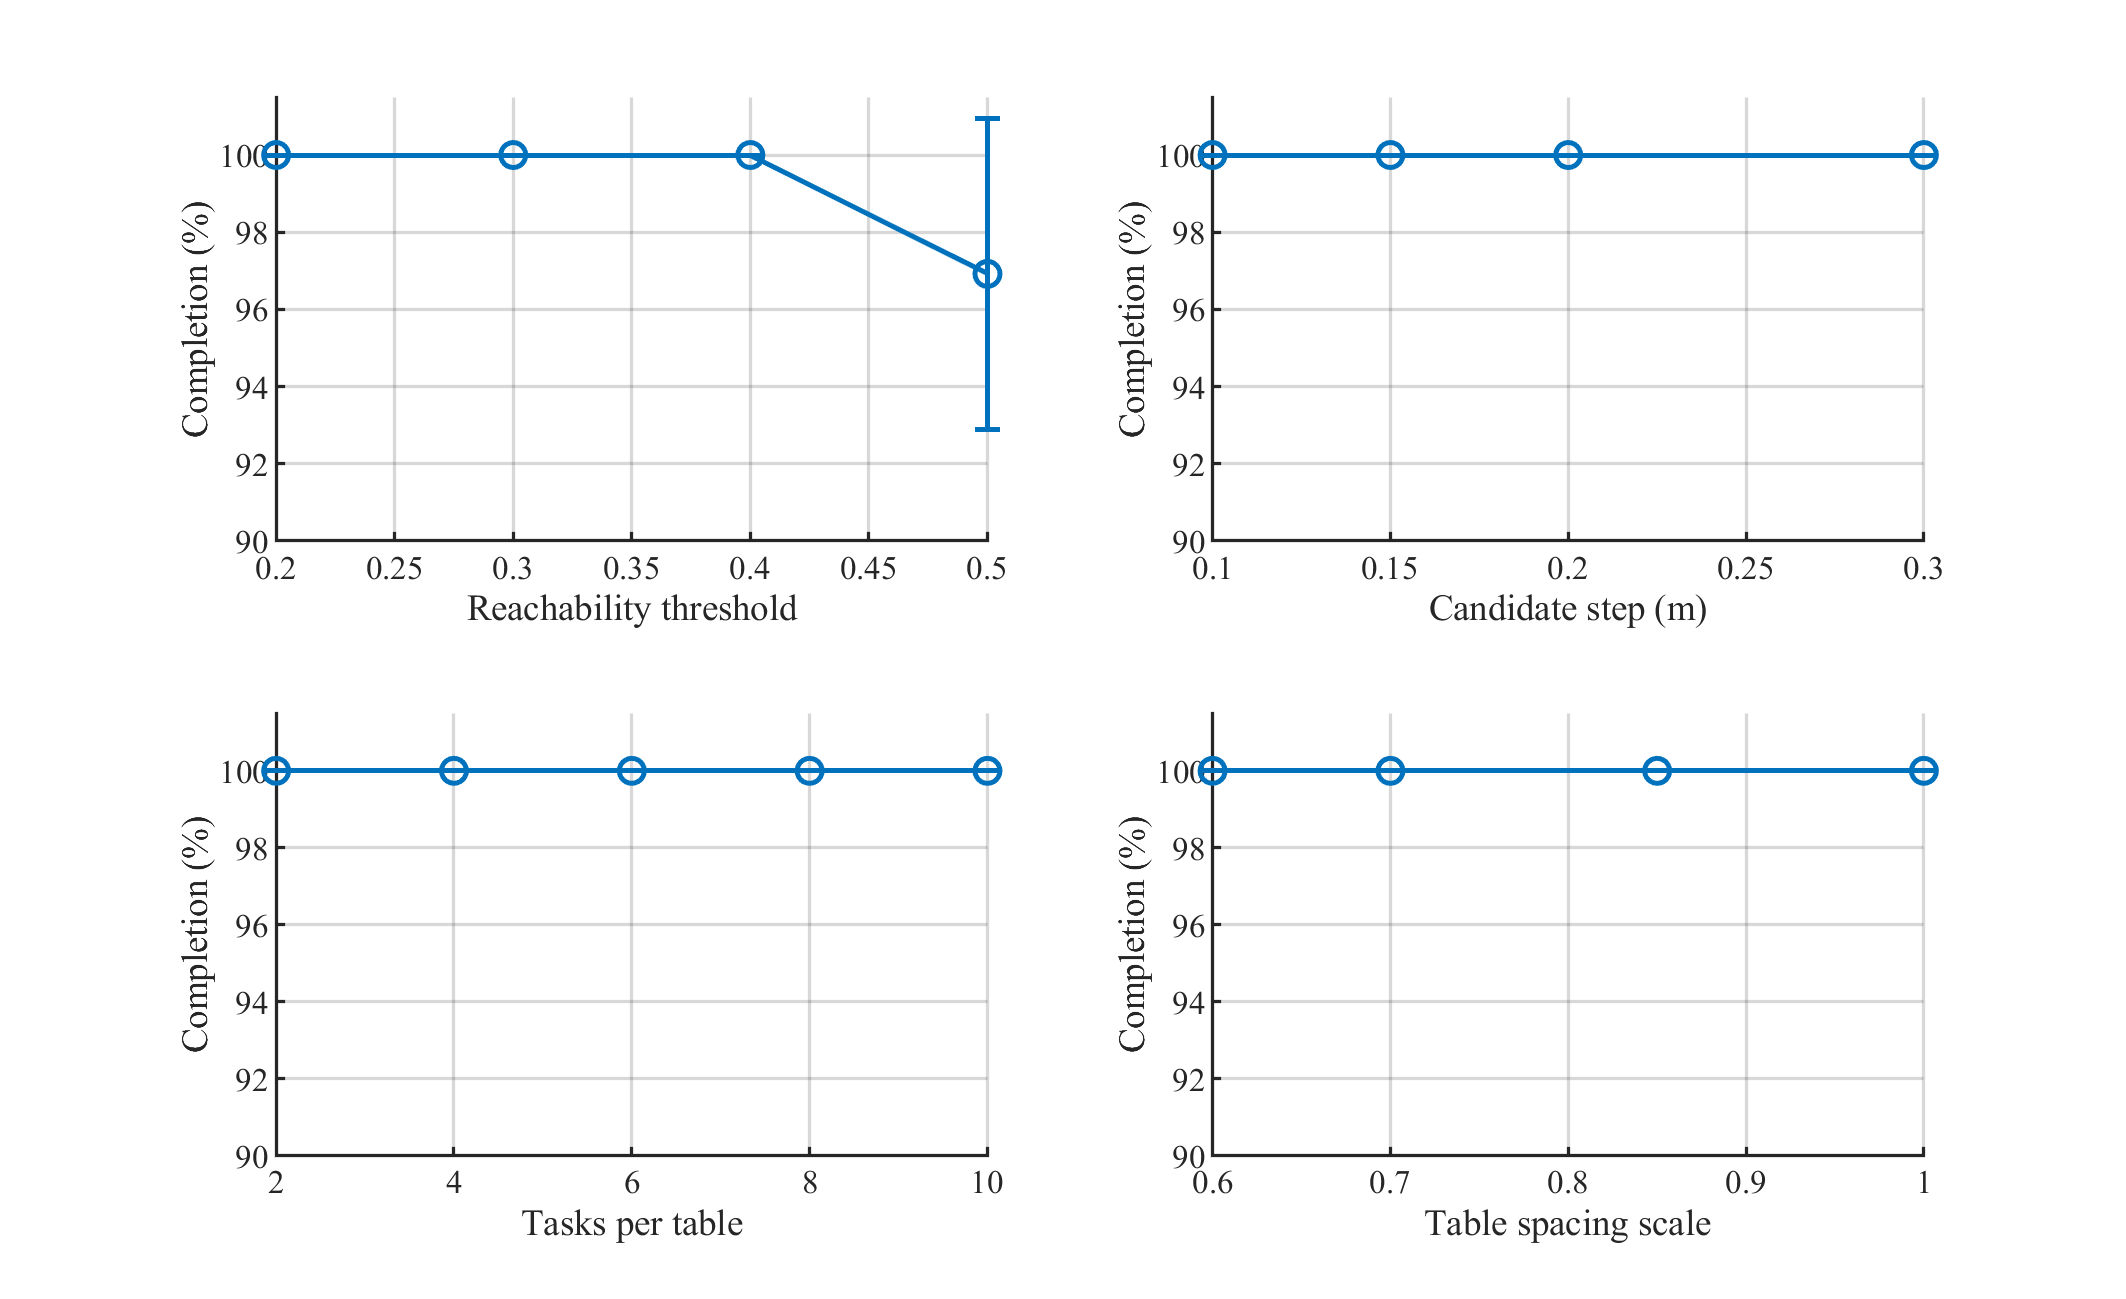
\includegraphics[width=\linewidth]{results/figures/tac_submission/png/fig_stress_boundary.png}
        \vspace{0.2em}
        \small (b) Boundary and sensitivity scans.
    \end{minipage}
    \caption{Robustness under difficult task distributions and parameter stress. 
    The full method remains stable across hard scenarios, while tighter reachability 
    constraints are the main source of completion degradation in the stress scan.}
    \label{fig:hard_stress}
\end{figure*}

\subsection{Runtime Scaling and Noise Robustness}
Figure~\ref{fig:runtime_routing1}(a) shows planning-time trends across scale and candidate-density settings.
 Planning time ranges from 1.92 s to 60.02 s in the submission summary, 
 consistent with the \(O(KN)\) candidate-evaluation term and the \(O(Q^2 C_{\Pi})\) pairwise path-cost term in Proposition~\ref{prop:complexity}.
  Figure~\ref{fig:runtime_routing1}(b) reports perturbation tests. 
  The full method's final completion ranges from 69.03\% to 100.00\% across noise settings,
   while the nearest-docking baseline remains at 0.00\% in the same summary.


\subsection{Global Planner Benchmark and Oracle Reference}
 Figure~\ref{fig:runtime_routing1}(c) compares global planners under the same selected docking sequence. 
 All seven planners succeed, with path-length and turn-count differences reflecting 
 the routing module rather than the docking selection module.
 A* gives 63.29 m, JPS gives 63.24 m, GBFS gives 66.47 m, Theta* gives 62.46 m, Lazy Theta* gives 62.87 m, 
 and Convex A* gives 63.29 m in the fixed-order benchmark. 
 Figure~\ref{fig:runtime_routing1}(d) compares the heuristic with a small-scale bounded candidate-set oracle. 
 The relative gap ranges from -4.56\% to 0.63\%; 
 negative gaps arise from the restricted comparison objective and 
 should be interpreted as a consistency check rather than a proof of global optimality. 

% \twocolumn[{
%     \begin{center}
%     \begin{minipage}[t]{0.49\textwidth}
%         \centering
%         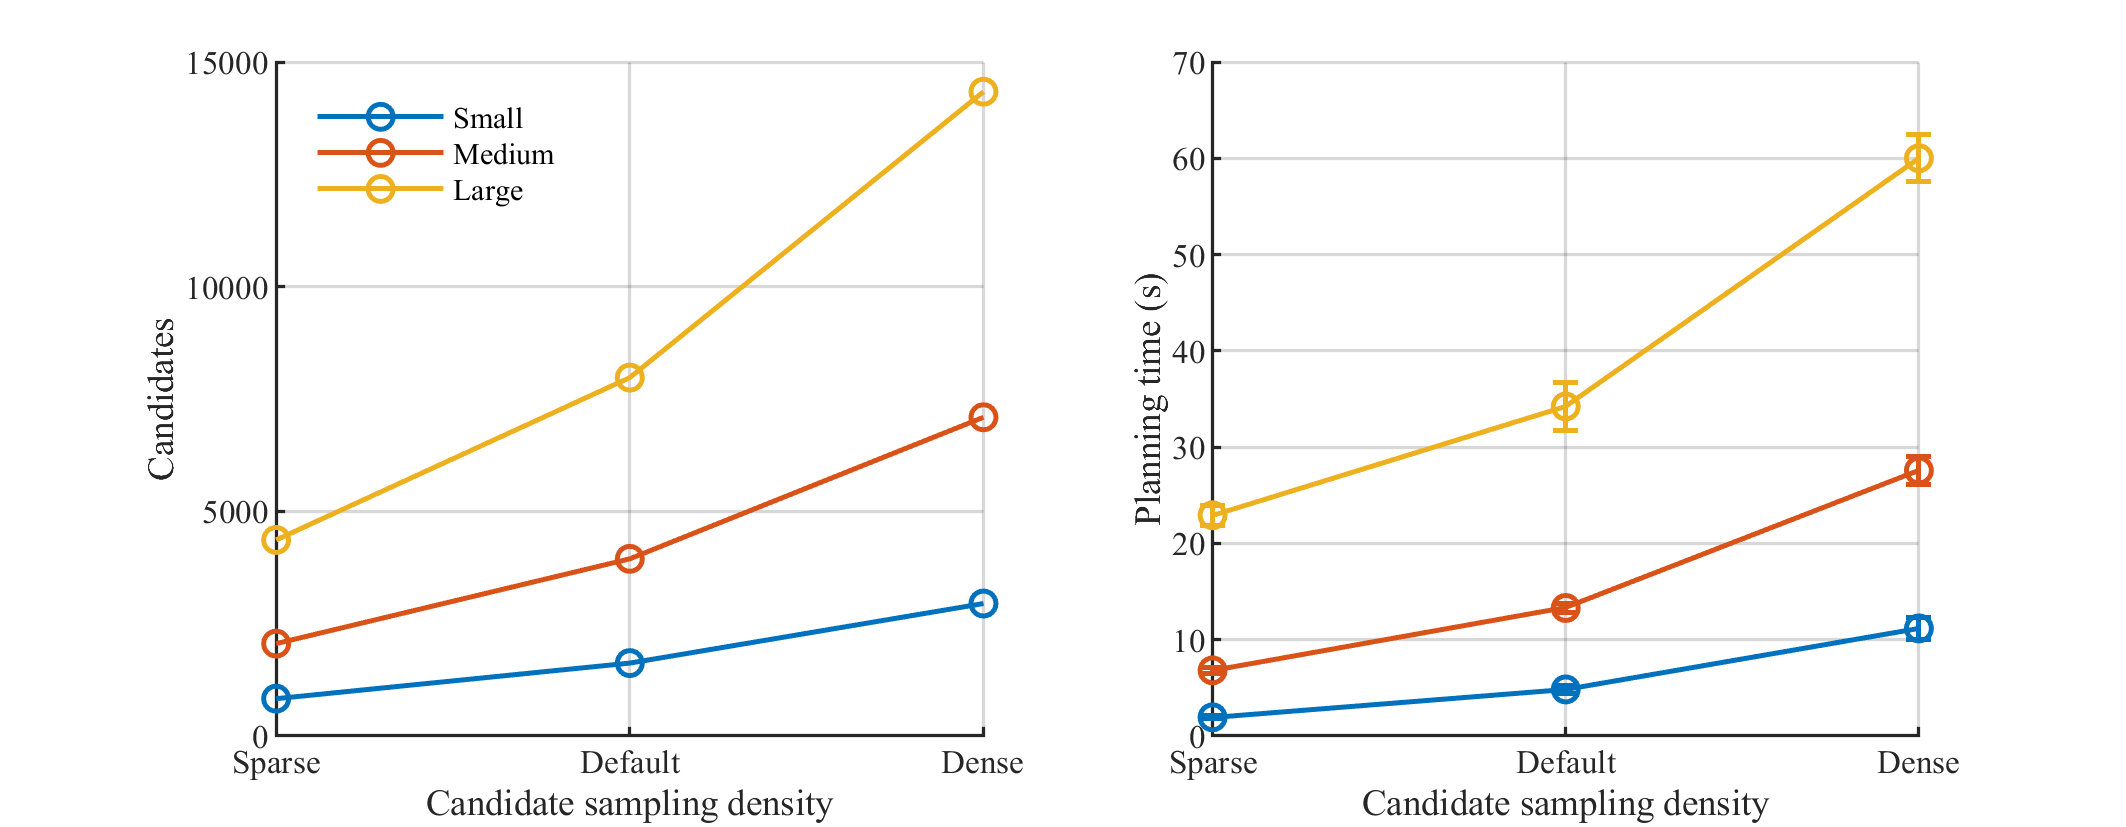
\includegraphics[width=\linewidth]{results/figures/tac_submission/png/fig_runtime_scaling.png}
%         \vspace{0.2em}
%         \small (a) Runtime scaling.
%     \end{minipage}\hfill
%     \begin{minipage}[t]{0.49\textwidth}
%         \centering
%         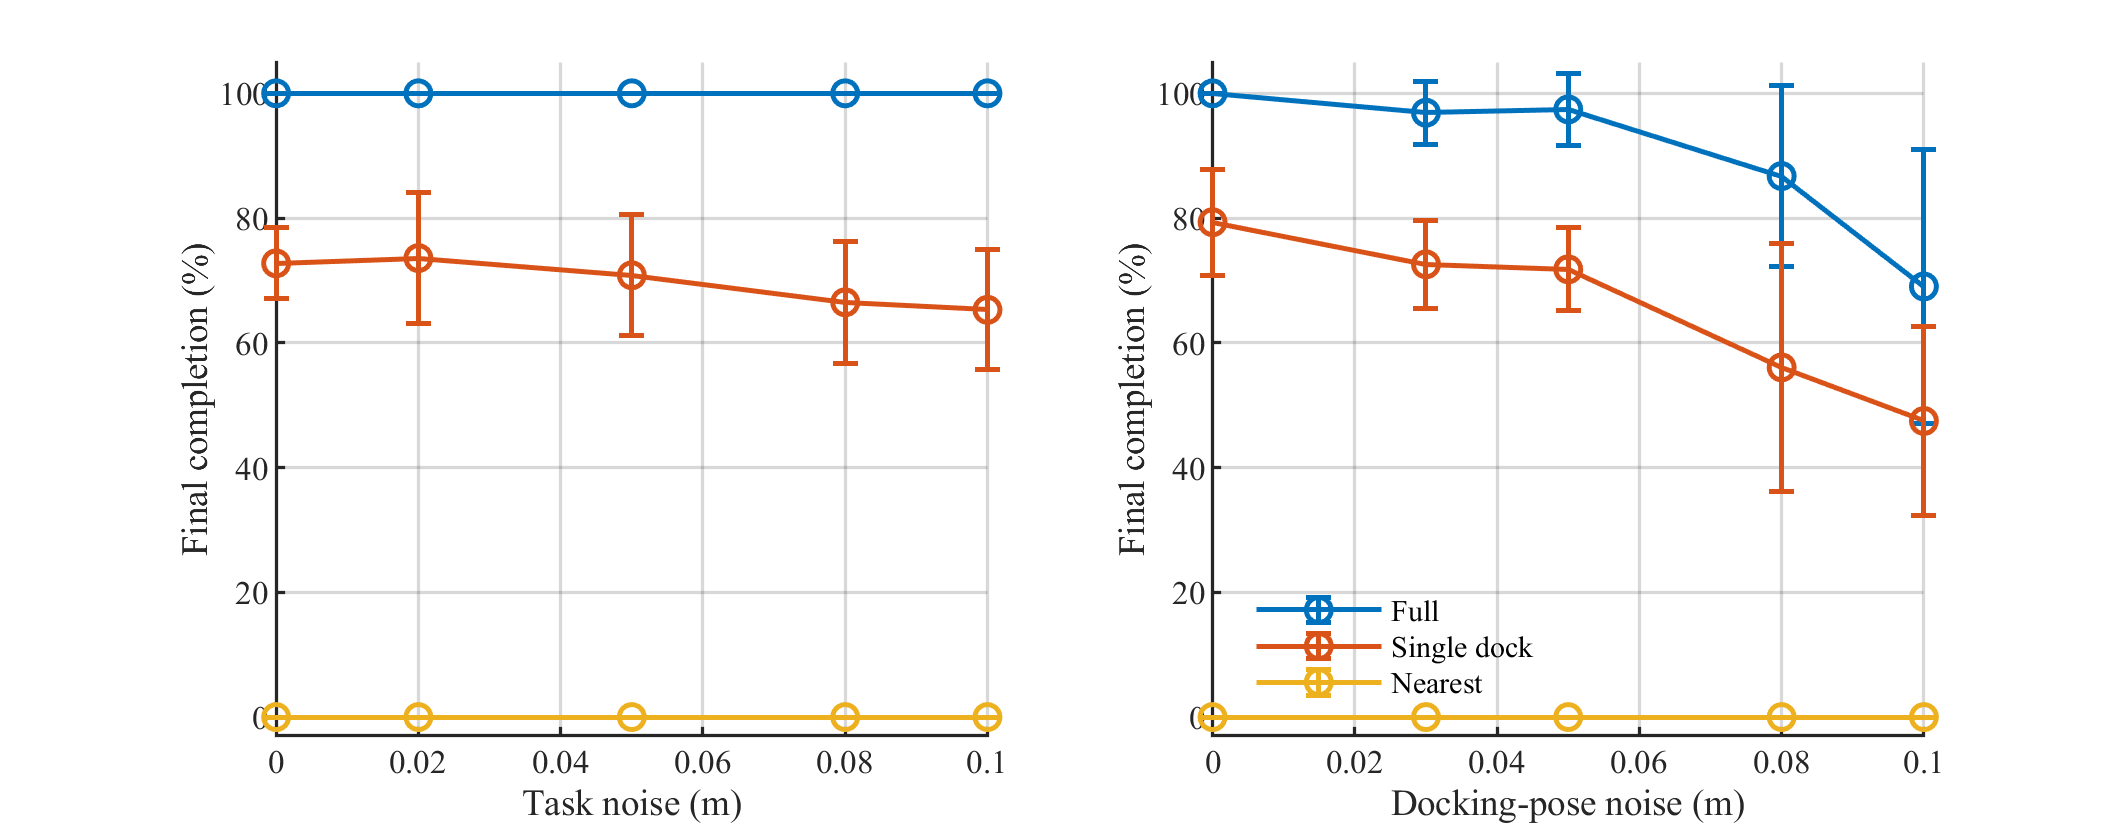
\includegraphics[width=\linewidth]{results/figures/tac_submission/png/fig_noise_robustness.png}
%         \vspace{0.2em}
%         \small (b) Noise robustness.
%     \end{minipage}
%     \vspace{0.5em}

%     \begin{minipage}[t]{0.49\textwidth}
%         \centering
%         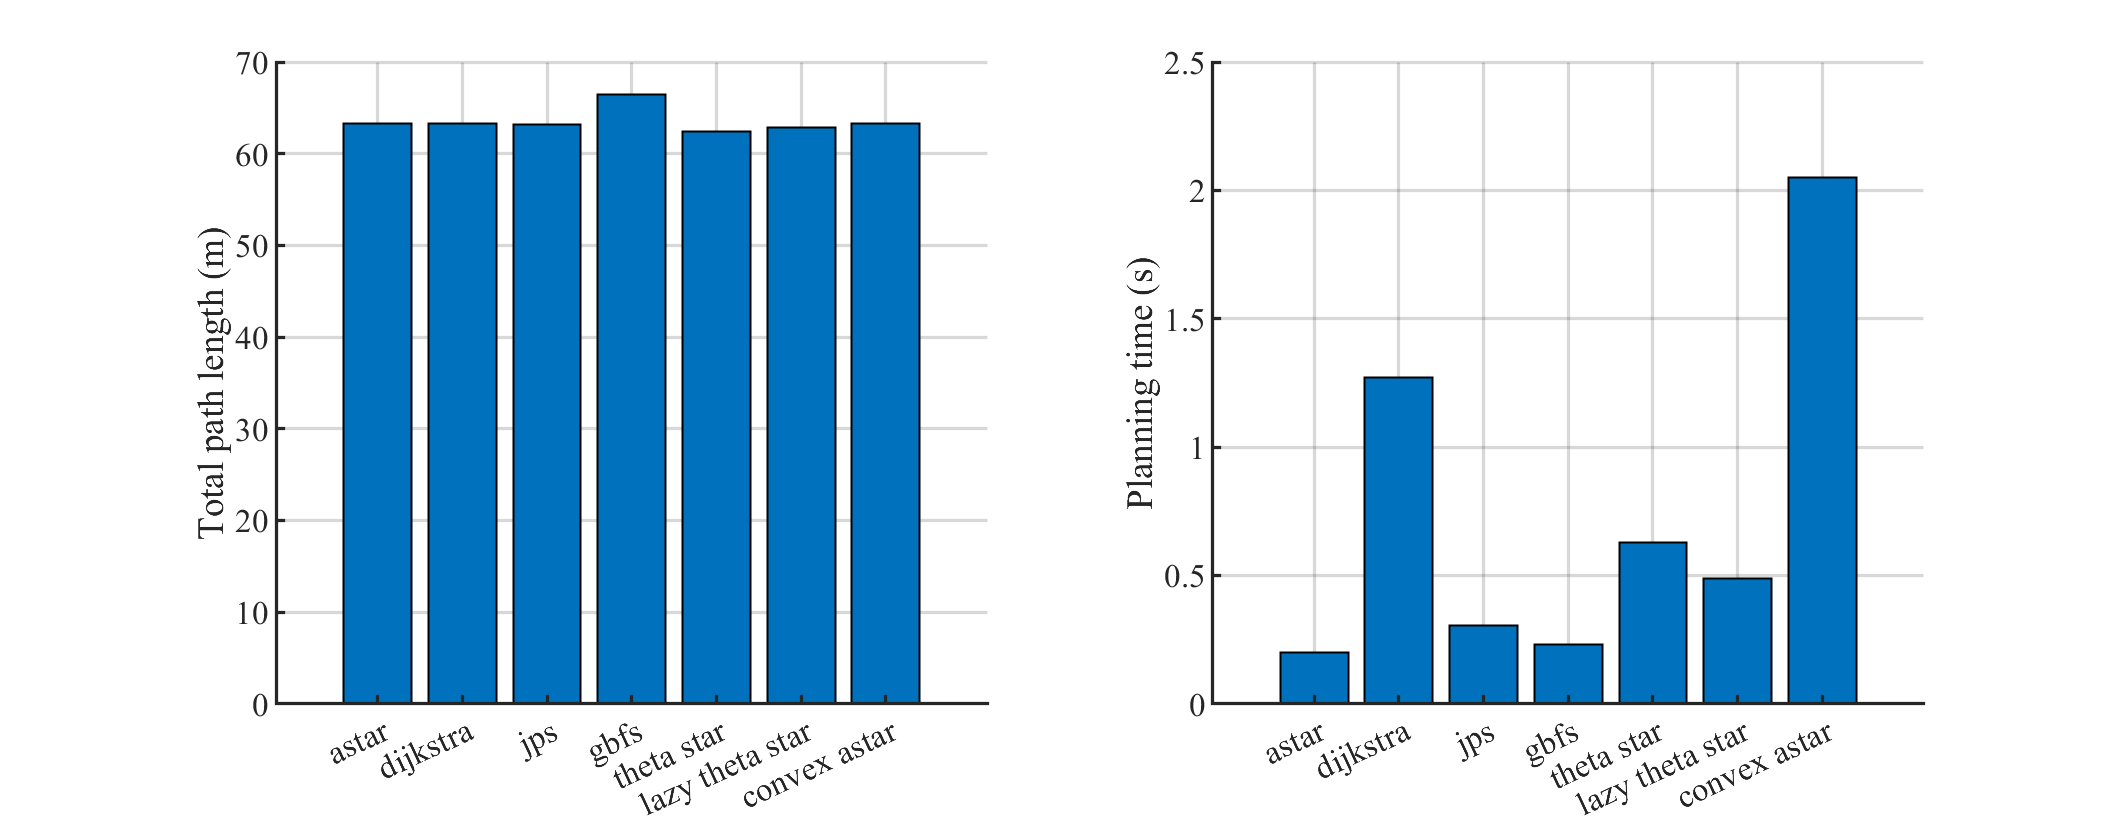
\includegraphics[width=\linewidth]{results/figures/tac_submission/png/fig_global_planner_benchmark.png}
%         \vspace{0.2em}
%         \small (c) Global planner benchmark.
%     \end{minipage}\hfill
%     \begin{minipage}[t]{0.49\textwidth}
%         \centering
%         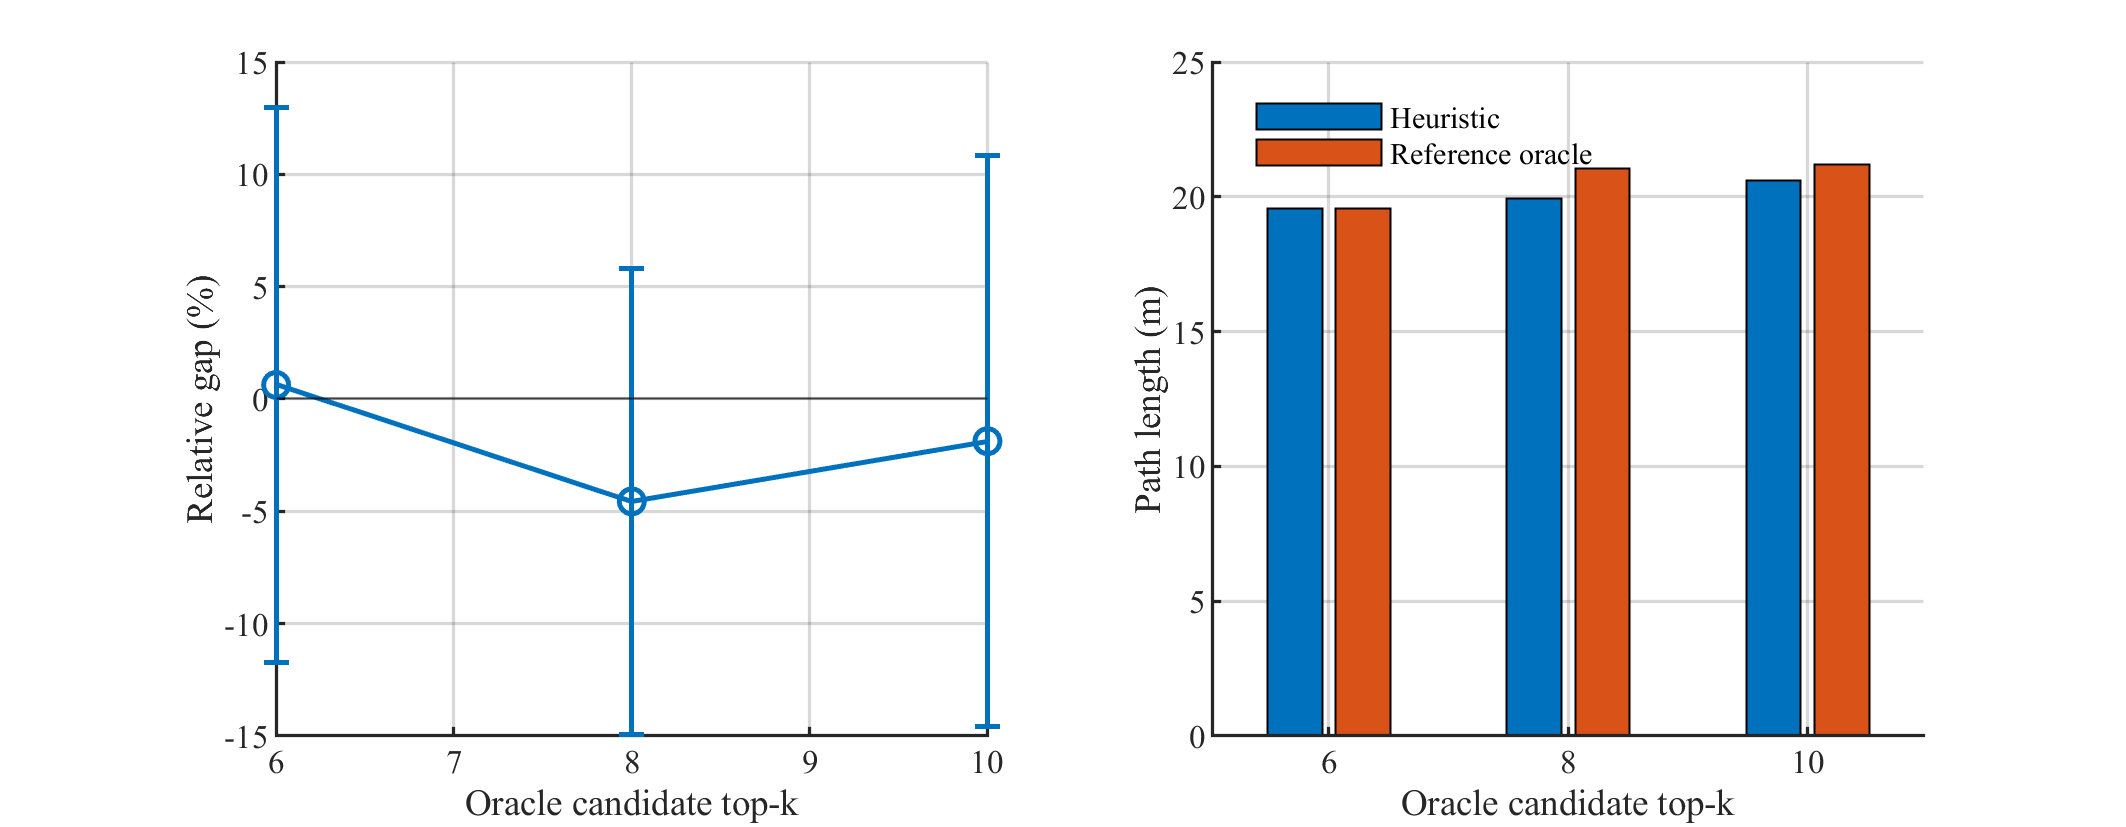
\includegraphics[width=\linewidth]{results/figures/tac_submission/png/fig_oracle_gap.png}
%         \vspace{0.2em}
%         \small (d) Small-scale oracle reference.
%     \end{minipage}
%     \refstepcounter{figure}\label{fig:runtime_routing}
%     \vspace{0.3em}

%     \parbox{0.96\textwidth}{\footnotesize \textbf{Fig.~\thefigure.} 
%      Runtime, perturbation, routing, 
%      and oracle-reference results. Runtime increases with scene scale and candidate density; 
%      reachability-aware coverage improves robustness under perturbations; 
%      changing the global planner affects route properties without changing docking selection;
%      and the heuristic remains close to the bounded candidate-set oracle on reduced instances.}
%     \end{center}
%     \vspace{0.6em}
% }]

\begin{figure*}[!t]
    \centering
    \begin{minipage}[t]{0.49\textwidth}
        \centering
        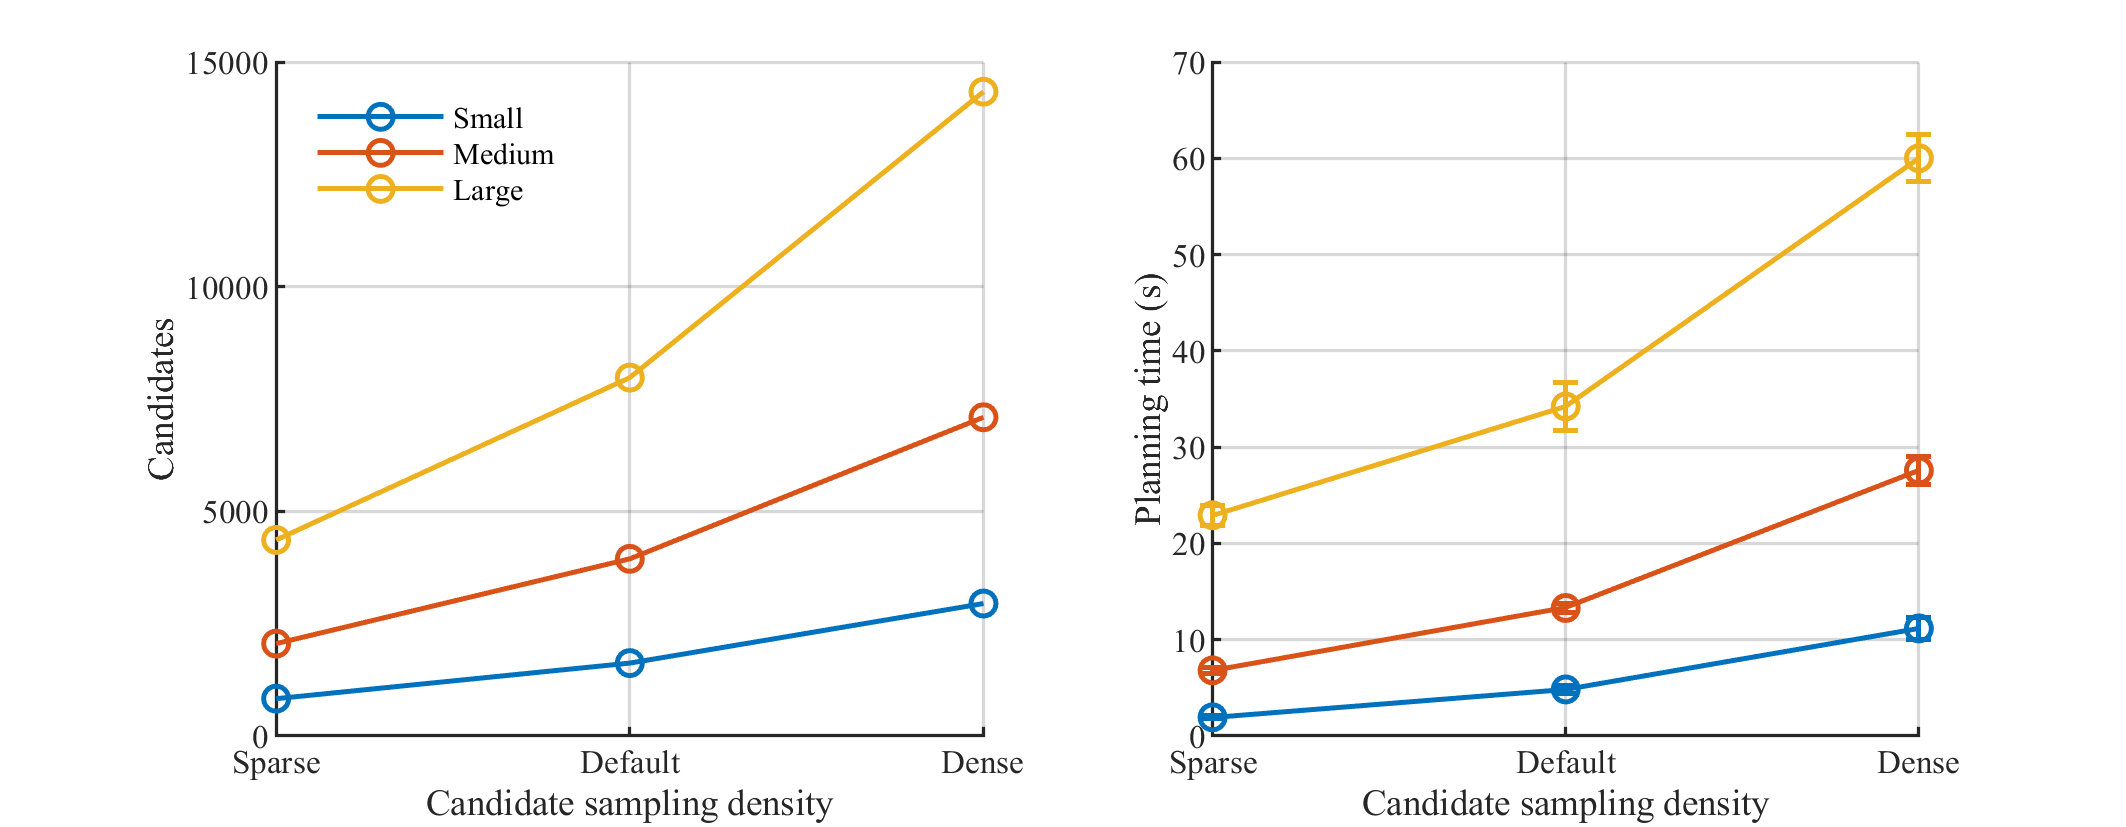
\includegraphics[width=\linewidth]{results/figures/tac_submission/png/fig_runtime_scaling.png}
        \vspace{0.2em}
        \small (a) Global planner benchmark.
    \end{minipage}\hfill
    \begin{minipage}[t]{0.49\textwidth}
        \centering
        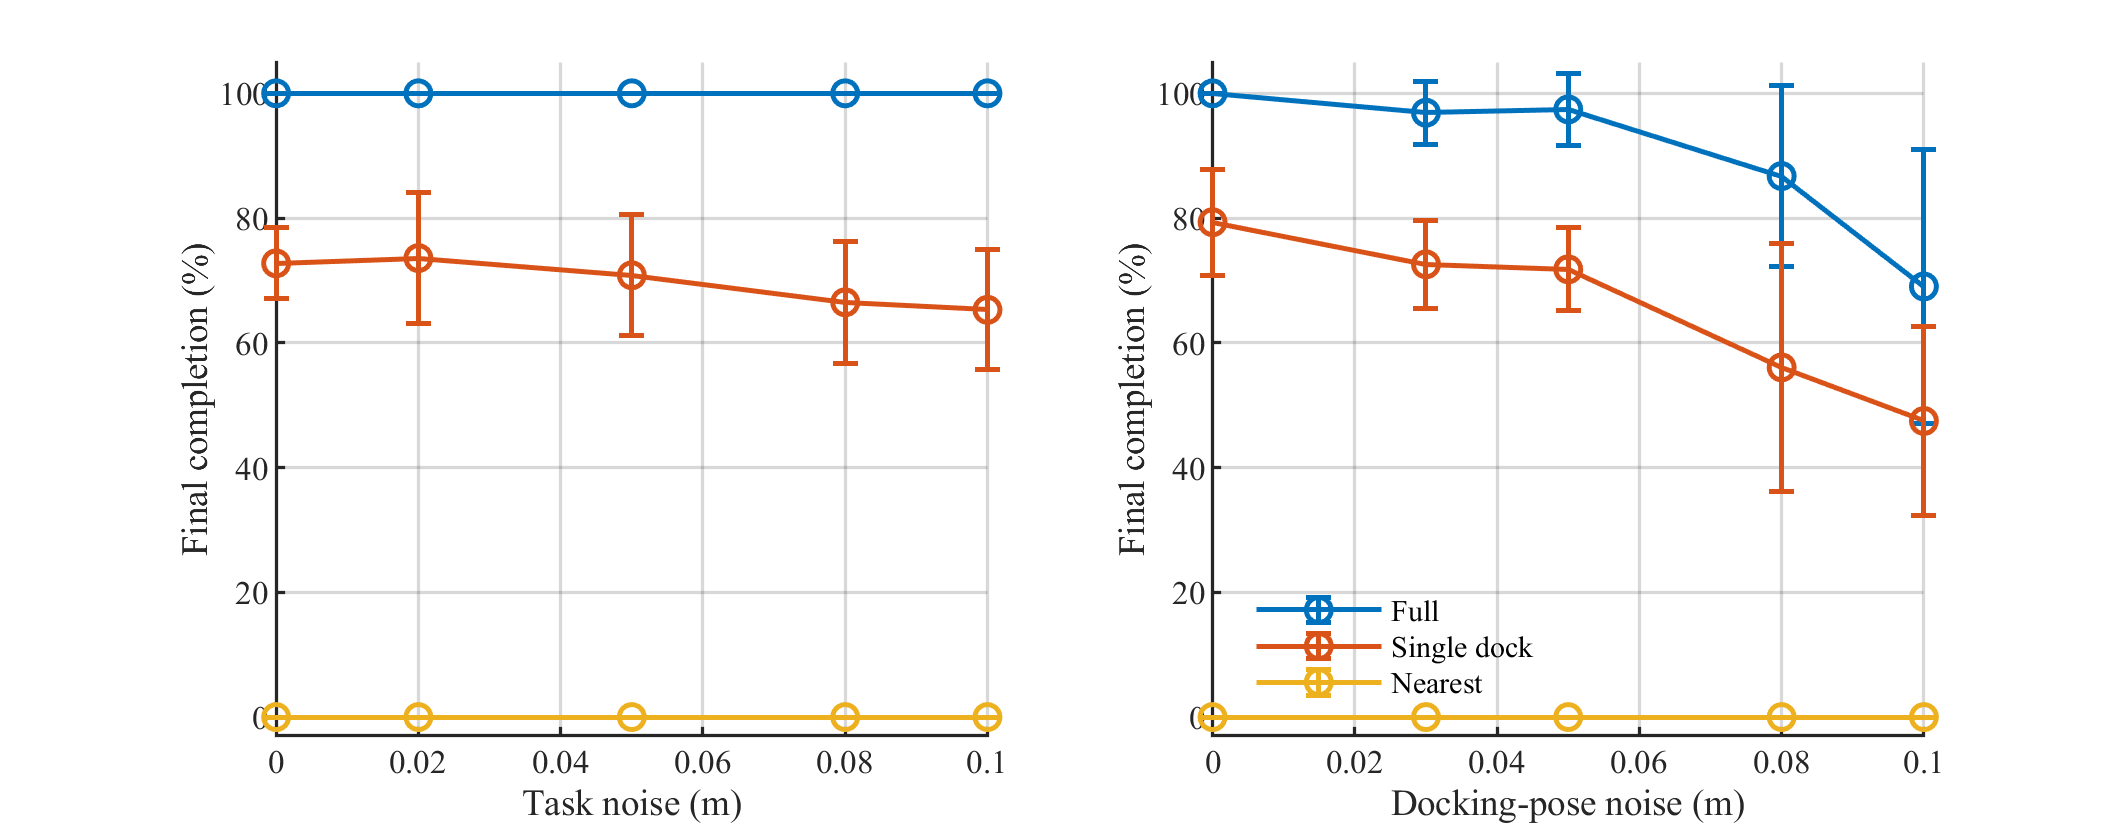
\includegraphics[width=\linewidth]{results/figures/tac_submission/png/fig_noise_robustness.png}
        \vspace{0.2em}
        \small (b) Small-scale oracle reference.
    \end{minipage}
    \caption{Robustness under difficult task distributions and parameter stress. 
    The full method remains stable across hard scenarios, while tighter reachability 
    constraints are the main source of completion degradation in the stress scan.}
    \label{fig:runtime_routing1}
\end{figure*}

\begin{figure*}[!t]
    \centering
    \begin{minipage}[t]{0.49\textwidth}
        \centering
        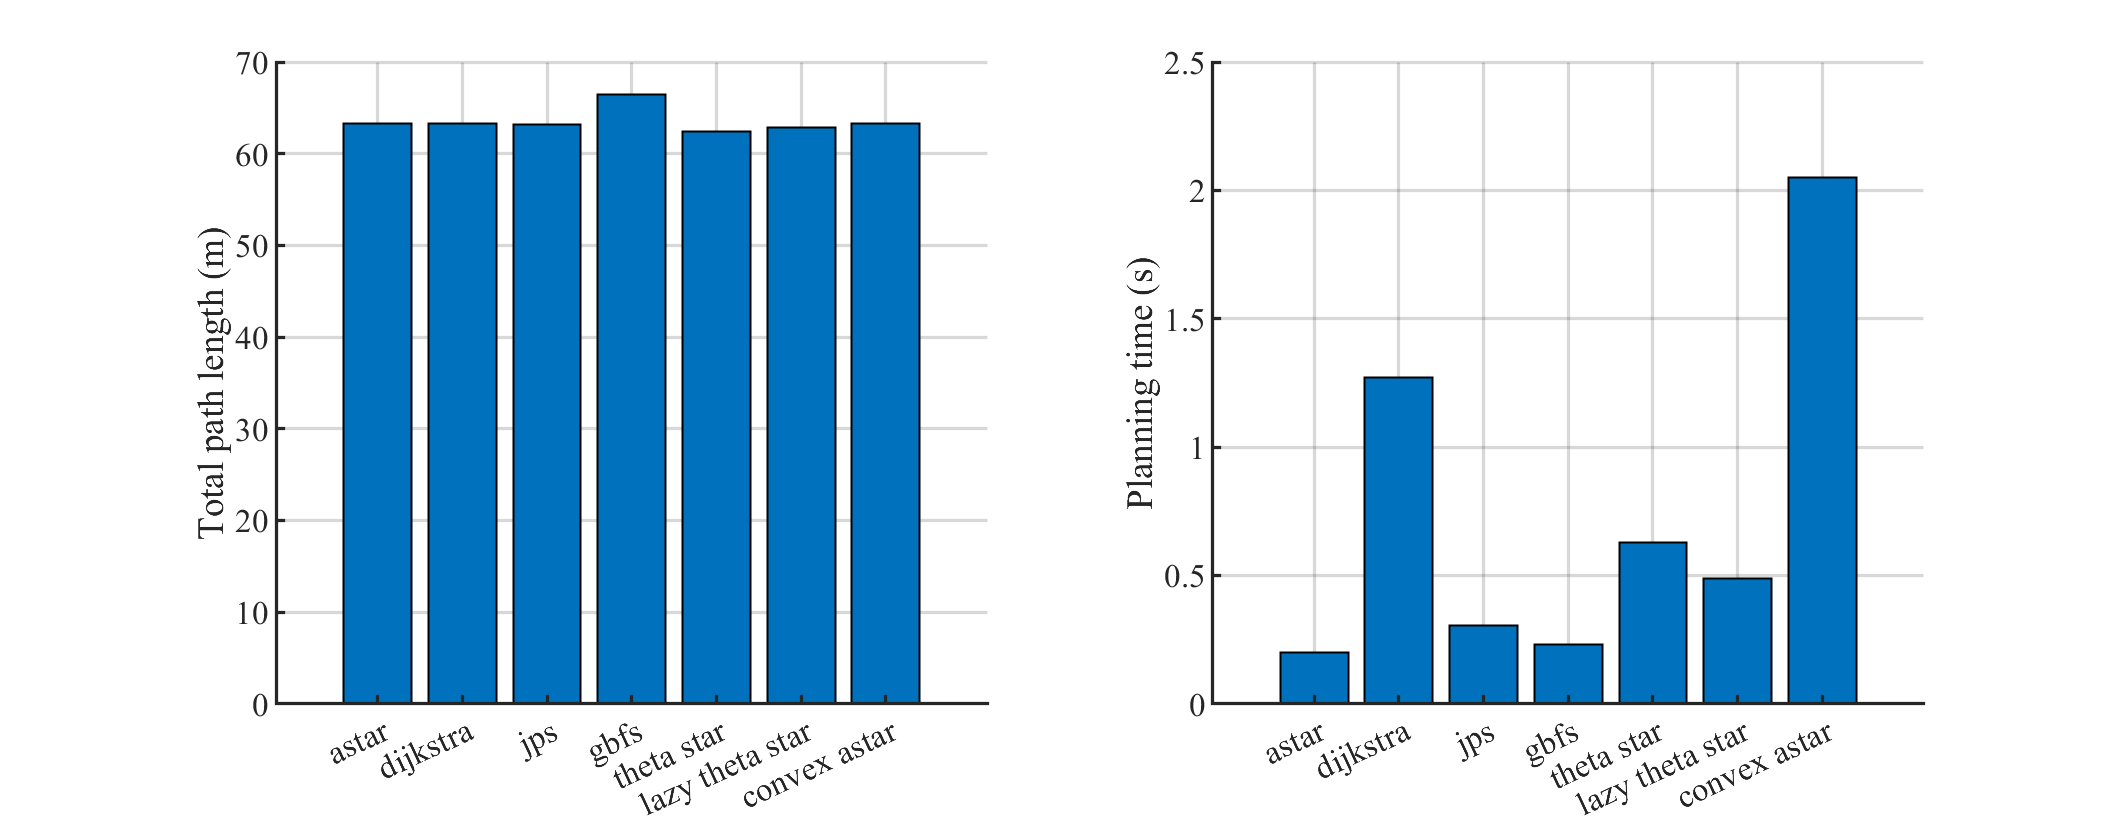
\includegraphics[width=\linewidth]{results/figures/tac_submission/png/fig_global_planner_benchmark.png}
        \vspace{0.2em}
        \small (a) Global planner benchmark.
    \end{minipage}\hfill
    \begin{minipage}[t]{0.49\textwidth}
        \centering
        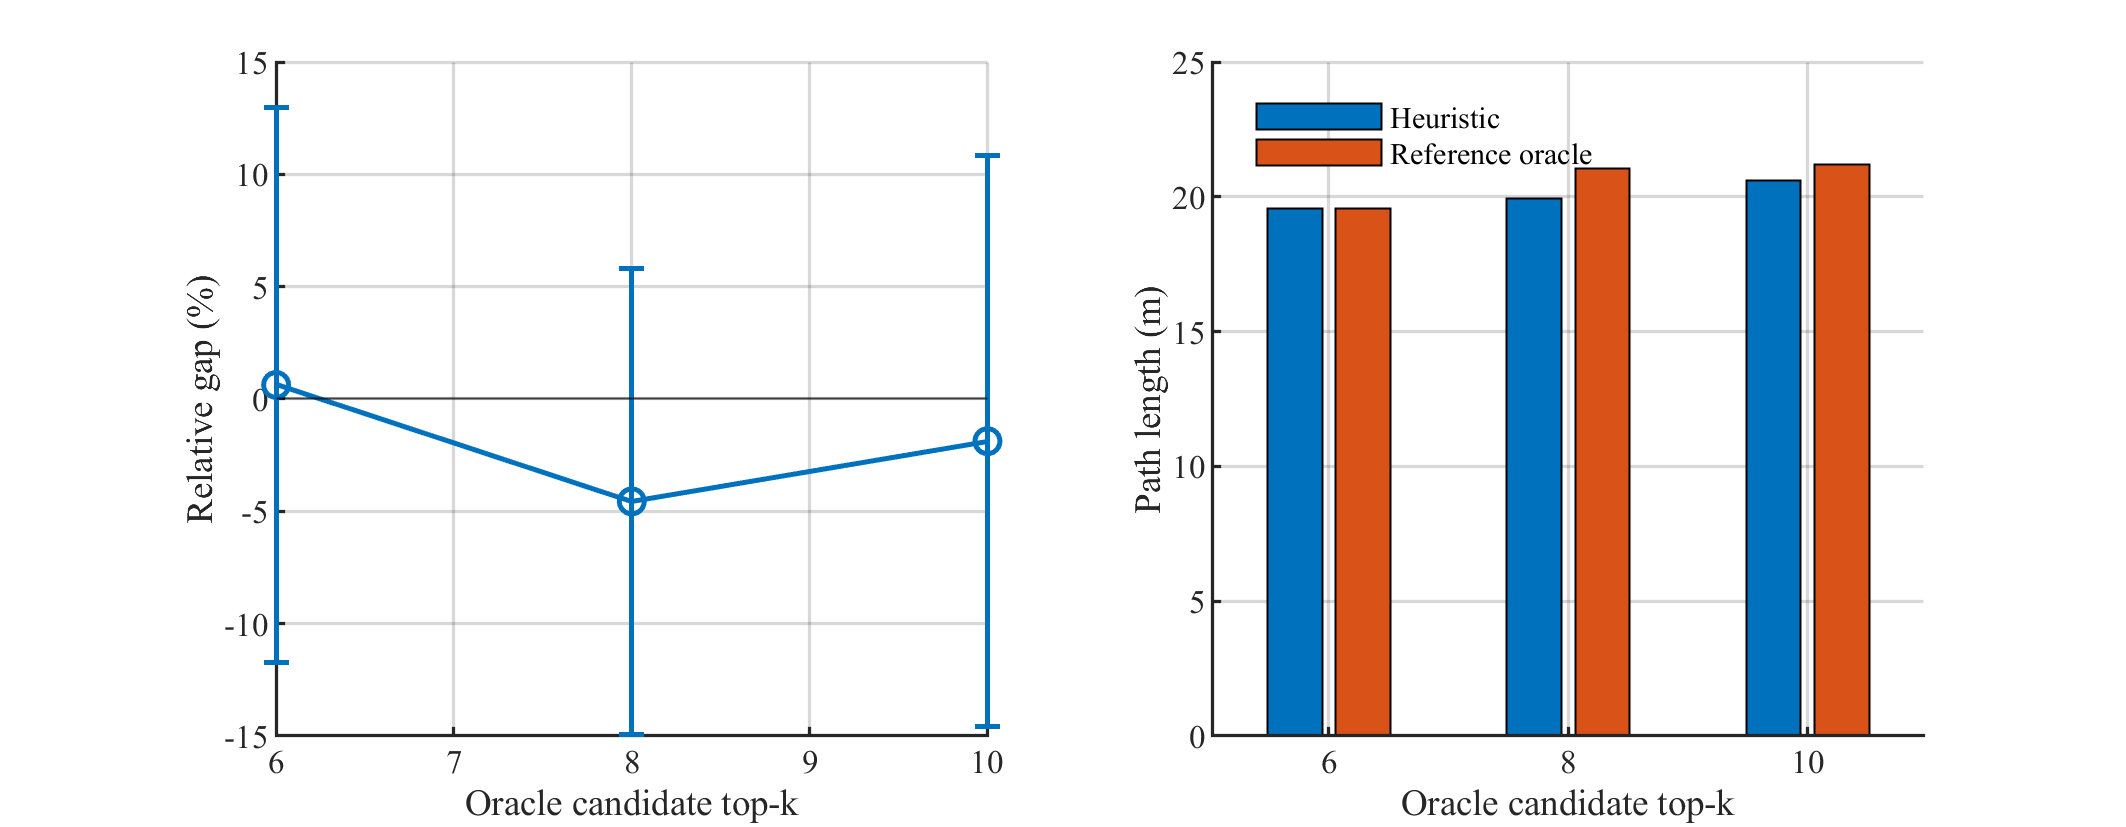
\includegraphics[width=\linewidth]{results/figures/tac_submission/png/fig_oracle_gap.png}
        \vspace{0.2em}
        \small (b) Small-scale oracle reference.
    \end{minipage}
    \caption{Robustness under difficult task distributions and parameter stress. 
    The full method remains stable across hard scenarios, while tighter reachability 
    constraints are the main source of completion degradation in the stress scan.}
    \label{fig:runtime_routing2}
\end{figure*}



